%!TEX root = Thesis.tex

\newcommand\Bx{x}
\newcommand\Bm{m}
\def\v{\vm{v}}
\newcommand\vm[1]{\bm{\mathrm{#1}}}
\renewcommand{\v}{{\mbox{a}^i}}
\newcommand{\z}{z_{t}}
\newcommand{\y}{z_{1:t-1}}

\chapter{In-vehicle parking space occupancy estimation and guidance system}
\label{cha:our_approach}

\section{Overview} % (fold)
\label{sec:overview}

In this chapter, we describe in detail the three main components of our proof
of concept system prototyped for in-vehicle sensor setup: visual car
detection, creation of the map of parking lots capable to store their
occupancy information and a planner able to find a free parking lot in the
minimum expected time. We also present the way of integrating these parts into
a single consistent framework.

We start by a coarse outline of these different sections and present each of
these sub-parts in detail later in the chapter.

\begin{itemize}

\item \emph{Perception:}  We visually detect cars in the images taken from the
stereo camera and estimate how far from the image plane are they situated by
fusing the detections with the depth data, received either from the stereo
disparity or from the laser range finder (Section~\ref{sec:perception}).

\item \emph{Parking Lots Modeling:}  The positions of the detected cars are
fused into one global representation of the world observed by the agent. This
representation also contains occupancy information, perceived through multiple
runs (Section~\ref{sec:model}).

\item \emph{Planning:}  In the modeled environment we search for actions that
minimize the expected time spent on searching for a parking space and walking
from it to the goal (Section~\ref{sec:action_planning}).

\end{itemize}

% section overview (end)

\section{Perception} % (fold)
\label{sec:perception}

We start by motivating the choice of the visual detection framework. There is
a number of object detection methods to choose from. We investigate three
different approaches, utilizing different visual features: Haar features,
local binary patterns (LBPs) and histograms of oriented gradients (HOGs).

\citet{violajones2001} introduce the Haar feature based object detection.
Their approach provides the detection rate of up to 95\% when applied to face
detection. The main drawback of the proposed method for our setup is that it
suffers from the changes in the shape of the object, rotations, occlusions and
from the illumination changes. For the task of car detection it is important
to allow for a certain degree of deviation for the reason that the cars can
differ in shape and angle from which they are observed. They also can be
occluded by people walking in front of them or other cars. In addition to
these variations, we may also observe them in different lighting conditions.

Utilizing the local binary patterns (LBPs) as presented by~\citet{lbp2010}
addresses the illumination issues and overall boosts the detection rates and
performance. It is, however, similarly to Haar features, vulnerable to
rotation and shape changes.

Moreover, to the extent of our knowledge, LBP-based methods are slow on the
training stage. Despite, not being a crucial measure of an algorithm
performance, the training time is still an important argument, as it
influences the usability of the method, especially on implementation stage.

Throughout the development of this thesis, we tried all these and finally
decided to apply the HOG-based detector following the work
of~\citet{dalal2005}. It relies on the gradient-based features and is
therefore invariant to illumination and brightness changes. Additionally, the
presented method stays robust to slight changes in rotation and shape.

\subsection{HOG Detector}\label{sub:hog_detector}

The HOG representation has several relevant properties for the problem under
consideration. It captures edge or gradient structure that is very
characteristic of local shape, and it does so in a local representation with
an easily controllable degree of invariance to local geometric and photometric
transformations: translations or rotations make little difference if they are
much smaller than the local spatial or orientation bin size.

\begin{figure}[th]
\centering
\subfloat[]{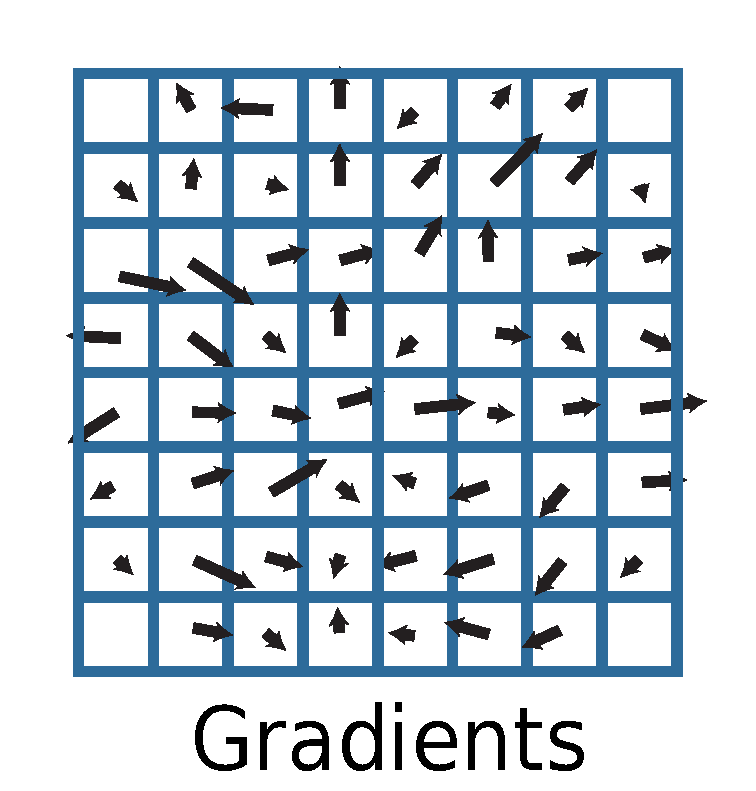
\includegraphics[width=0.27\textwidth]{pictures/gradients.pdf}\label{subfig:gradient}} \hspace{3mm}
\subfloat[]{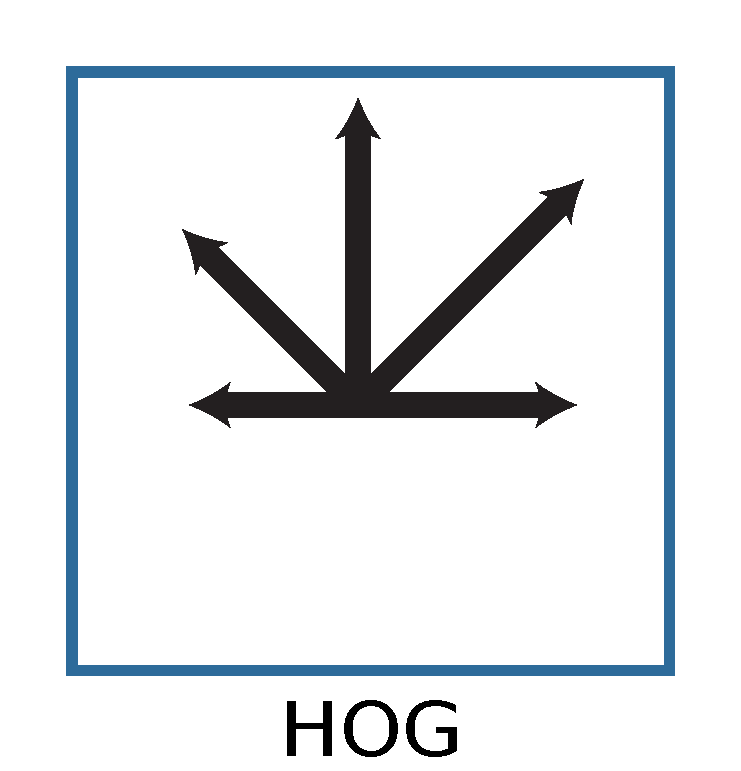
\includegraphics[width=0.27\textwidth]{pictures/hog.pdf}\label{subfig:hog}} \hspace{3mm}
\subfloat[]{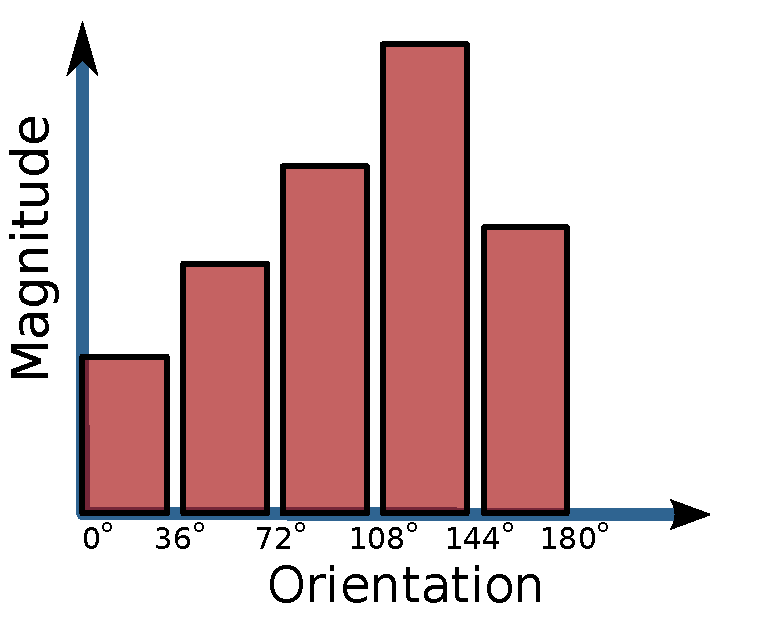
\includegraphics[width=0.4\textwidth]{pictures/hog_dist.pdf}\label{subfig:histogram}}
\caption{This figures shows gradient orientations for every pixel of the detection window \subref{subfig:gradient}, the corresponding histogram \subref{subfig:histogram} and its visualization \subref{subfig:hog}. The directions of the arrows in \subref{subfig:histogram} represent the angle covered by each bin, the lengths of arrows correspond to the magnitude of the gradients that fall into the corresponding bin. In this example, for better visualization, the histogram consists of 5 values, covering the range of $180^\circ$, meaning that each bin covers the angle of $36^\circ$, whereas the experiments in this thesis, use the histograms consisting of 9 bins.}
\label{fig:hog_simple}
\end{figure}

Following~\citet{dalal2005}, we make use of the histograms of oriented
gradients placed in a dense grid on the query images. The descriptor is
created by computing the gradient magnitude and orientation in each pixel of
the detection window and storing the orientations in a histogram. For each $8
\times 8$ pixel block in the image we form a histogram by assigning the
gradient orientations to distinct histogram bins, that cover all possible
orientation angles of the gradient. We do not take into account the direction
of the gradient vector, focusing only on its orientation. This allows for the
histogram bins to cover an angle of $180^{\circ}$ instead of $360^{\circ}$ to
ensure storing all possible orientations. A visualization of an example
histogram can be seen in Figure~\ref{fig:hog_simple}.

\begin{figure}[b]
 \centering
\subfloat[]{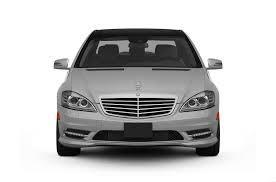
\includegraphics[width=0.31\textwidth]{pictures/original.jpg}\label{subfig:original}} \hspace{3mm}
\subfloat[]{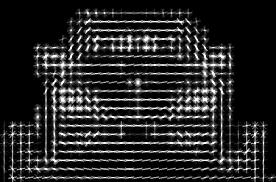
\includegraphics[width=0.31\textwidth]{pictures/glyph.jpg}\label{subfig:glyph}} \hspace{3mm}
\subfloat[]{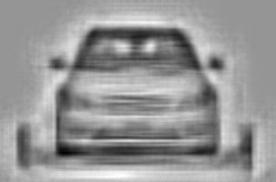
\includegraphics[width=0.31\textwidth]{pictures/ihog.jpg}\label{subfig:ihog}}
\caption{This figure shows a car image \subref{subfig:original}, a visual representation of the histogram values \subref{subfig:glyph} and a HOG inversion image from HOGles \cite{vondrick2013hoggles} \subref{subfig:ihog}.}
\label{fig:hog_car}
\end{figure}

To detect the front and rear sides of the cars, we set the size of the hog
descriptor window to $128 \times 128$ pixels. The idea behind this decision is
based on generally square-like shape of the cars, when seen from front or
rear. A square drawn around the car contains higher percentage of useful
information in comparison to a rectangle. To detect the side of the car, the
descriptor window is changed to $128 \times 64$ pixels following the same
logic.

These window sizes yield the number of the histograms that fit inside each
window which is the number of $8 \times 8$ pixel blocks contained in the
descriptor window. This results in 256 histograms for front/rear view and 128
histograms for the side view.

\begin{figure}[t]%
\centering
\subfloat[]{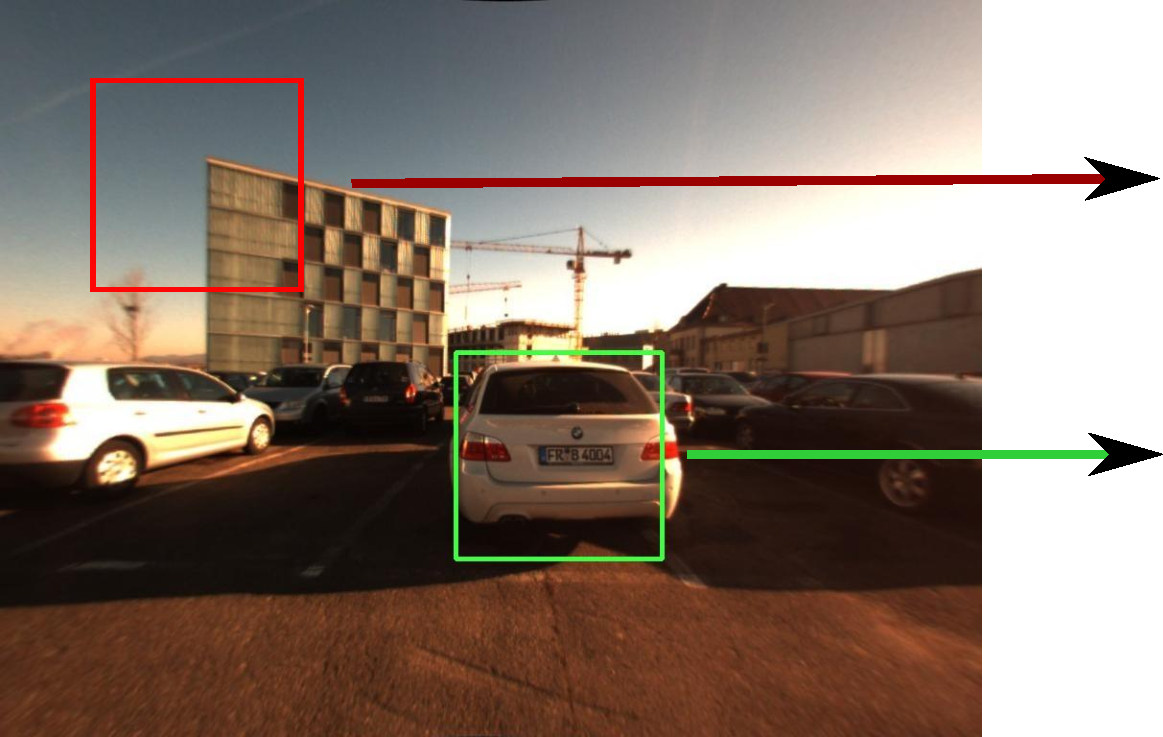
\includegraphics[width=0.6\textwidth]{pictures/detections.pdf}\label{subfig:hog_detector}}
\subfloat[]{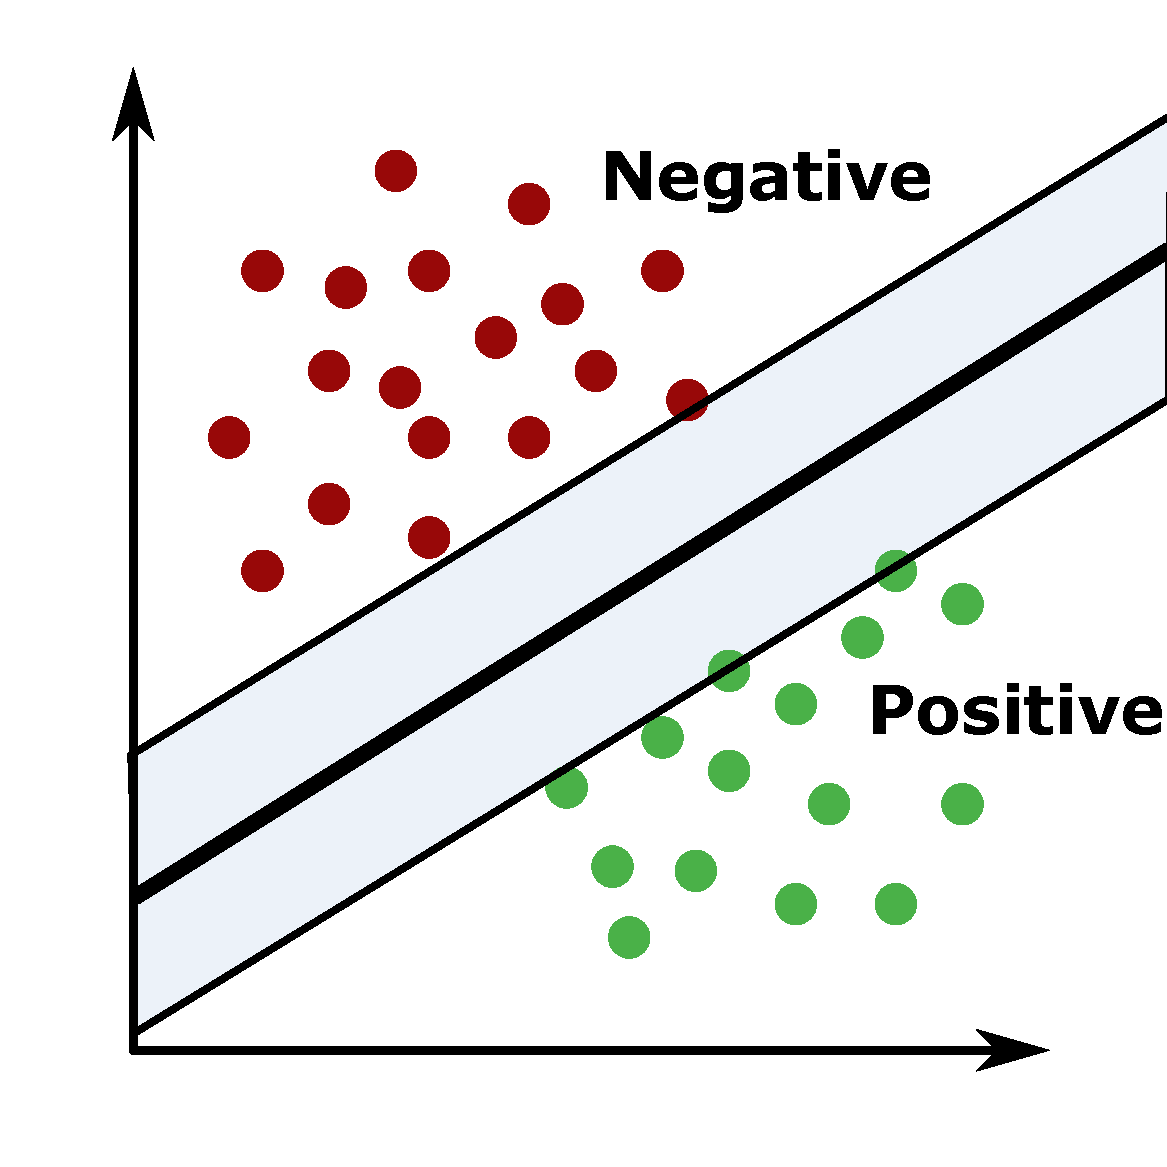
\includegraphics[width=0.4\textwidth]{pictures/svm.pdf}\label{subfig:svm_illustration}}
\caption{Illustration of HOG detection window~\subref{subfig:hog_detector} and clustering the corresponding multi-dimensional points via fitting a hyperplane using SVM~\subref{subfig:svm_illustration} which yields the maximal distance between the datasets.}
\label{fig:det_to_svm}
\end{figure}

We form a vector from all histogram values contained in each of 256 or 128
histograms that describe the detection window. Following~\citet{dalal2005}, we
consider that each histogram consists of 9 distinct bins. This results in the
vectors of sizes respectively 2304 and 1152 values for front/rear and side
view detection windows. We view this vector as a point in the space of same
dimensionality and seek for a hyperplane to classify these points into
positive and negative ones with the use of the support vector machines. This
is illustrated in Figure~\ref{fig:det_to_svm}.

% subsection hog_classifier (end)

\subsection{SVM Classifier}\label{sub:svm_classifier}

In order to carry out the decision in the test data, we train a linear Support
Vector Machines (SVM) classifier on top of all HOG descriptors. Alternatively,
a more complex decision boundary can be used, but linear SVM, despite its
simplicity, provides reasonable results. We show the detection performance in
the \nameref{cha:experimental_results} section.

\citet{svm} presented the support vector machines as a method to solve a two
class classification problem. For a dataset of points in $n$ dimensional space
SVM finds a hyperplane ($n-1$ dimensional plane) that optimally assigns them
to two classes maximizing the distance between the two resulting datasets. In
the linear SVM the decision boundary is linear.

SVM is a well-known and arguably the most popular algorithm in binary
clustering, therefore many implementations are readily available. In this work
we make extensive use of libSVM library by~\citet{libSVM2011}.

\begin{figure}[t]
    \begin{center}
        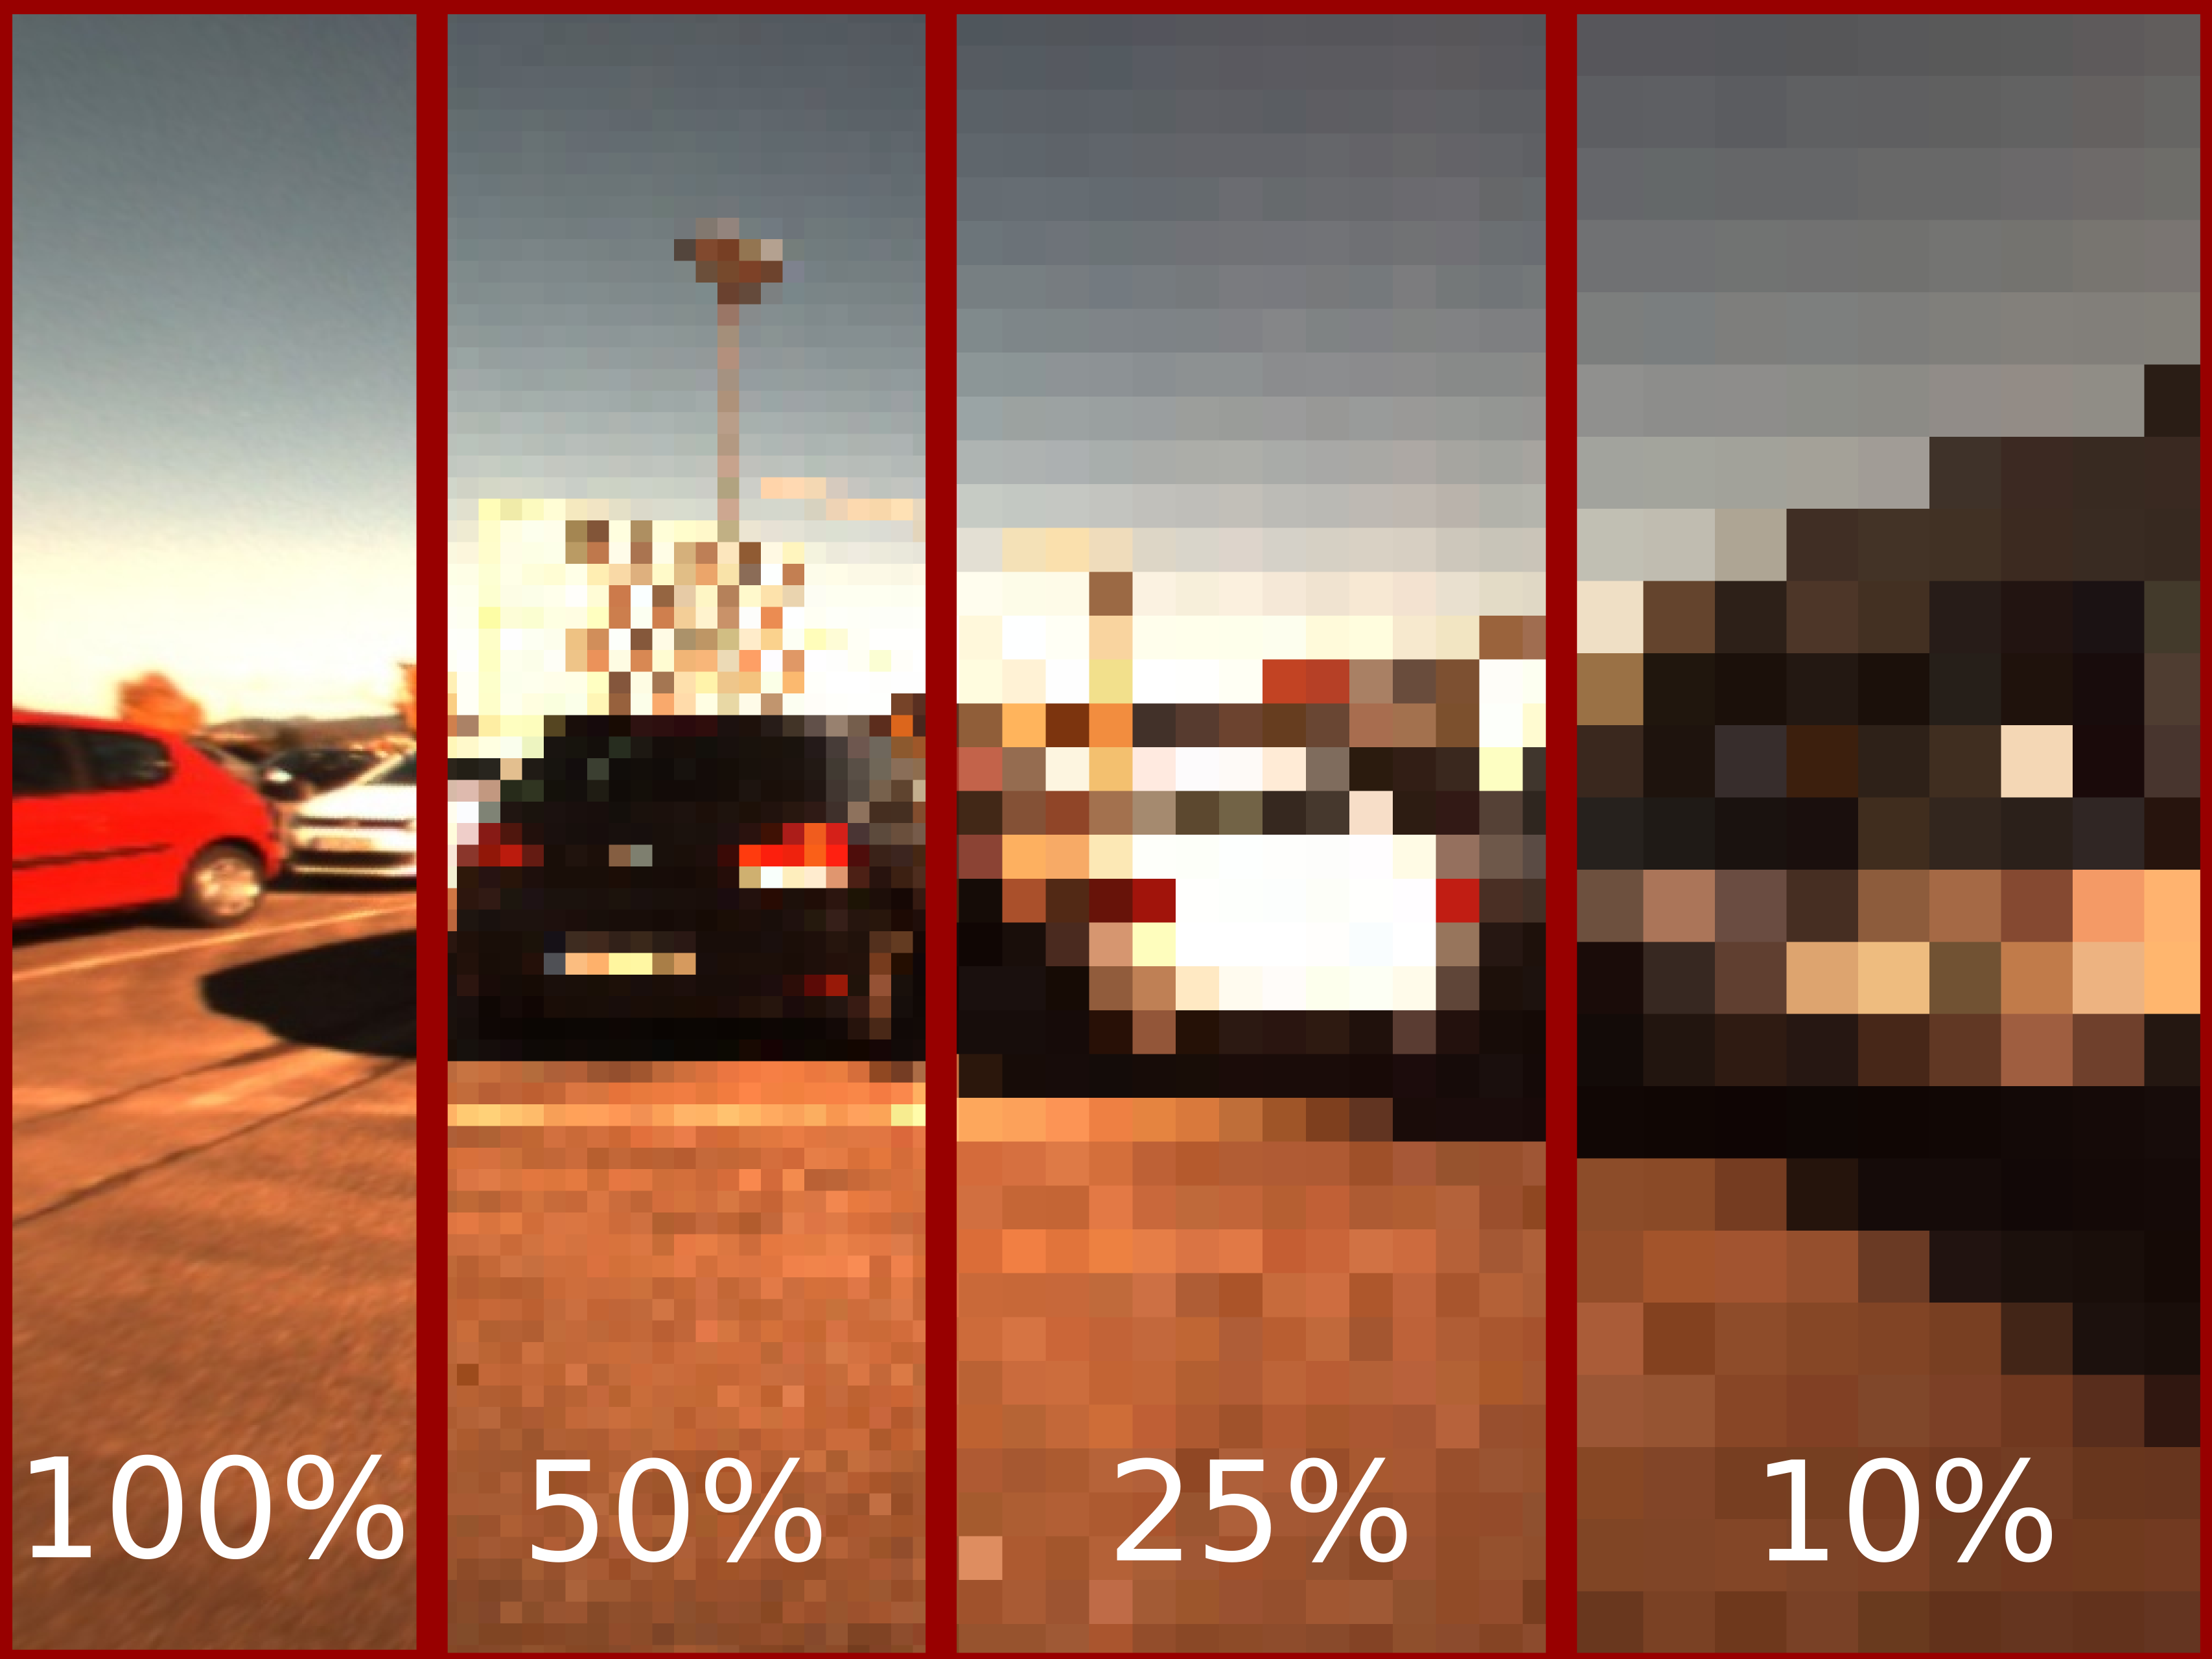
\includegraphics[width=0.6\textwidth]{pictures/cascades.png}
    \end{center}
    \caption{Each part of this figure illustrates a cut from the query image, sub-sampled with the corresponding scaling factor.}
    \label{fig:cascades}
\end{figure}

Based on the trained classifier, we carry out the detection in a cascade
fashion via the sliding window approach. That is: for every image we generate
a cascade which is effectively a set of images, sub-sampled with different
scaling factors. For every image in a cascade we slide a detection window of
the pre-defined size over the image. Every sliding window content yields a HOG
descriptor which we test against the pre-trained SVM classifier to find out to
which side of the decision boundary it is classified. If the current HOG
belongs to the side where the SVM has assigned the cars from the training
dataset then the current sliding window is a region of interest and contains a
car. We store each detection as a rectangle by saving the pixel positions of
the corners of the detection window around the car.

% subsection svm_classifier (end)

\subsection{Depth Information}\label{sub:depth_information}

In this section, we describe in details how the depth information is acquired
and combined with the visual detections described in the previous sections.

\subsubsection{Stereo Camera}\label{ssub:stereo_camera}

In order to find the depth from the stereo camera, we calculate the disparity
image from left and right images taken from the video stream. Knowing the
internal camera parameters we reconstruct the relative position of each pixel
of the disparity image.

The distance along the camera $z$ axis: $Z = \frac{fB}{d}$, where $f$ is the
focal length of the camera, $B$ is the baseline and $d$ is the disparity.
Given $Z$, we focus on finding $X$ and $Y$ coordinates from the projection
equations:

\begin{equation}
X = \frac{uZ}{f}
\hspace{10 mm}
Y = \frac{vZ}{f}
\end{equation}

where $u$ and $v$ are the pixel position in the $2D$ image and $X, Y, Z$ are
the $3D$ coordinates that correspond to the pixel $(u,v)$ in the camera frame.
$3D$ position that corresponds to every pixel in the image allows us to
combine depth information with visual detections.

Considering, that each detection is stored in the form of a region of interest
in the image coordinates, we are able to accumulate the depth of all pixels
that fall into it to estimate the joint depth of the detected car.

To find the distance to the car, we consider taking the median of all depth
values that fall into the corresponding region of interest. These depth values
contain high variance. The first reason for this is that they originate on the
surface of the car and the variance represents the difference in the distance
between different parts of the car. The second reason comes from the method in
which these depth values were acquired. The depth map from the stereo camera
setup proves to be noisy in the urban environments with homogeneous regions
like the sides or the hood of the car. Moreover parts of the environment are
seen through the windows of the car, adding additional noise to measurements.
An example can be found in Figure~\ref{fig:depth_from_disparity}.

This high variance of the input data results in the high uncertainty of the
precision in results' measurements. We further describe the method that uses
the laser range finder for the same task of finding the relative position of
the detected car to the camera.

% sub-subsection stereo_camera (end)
\subsubsection{Laser Range Finder}\label{ssub:laser_range_finder}

In order to use a laser range finder to detect the parked cars we used a
EUROPA robot Obelix which has a laser with an opening angle of $270^\circ$
mounted approximately on the human knee level. This setup proves to be more
robust in terms of finding the exact relative position of the detected car.

The laser mounted on the robot provides a sufficient opening angle to cover
the field of view of the camera. We search for the beams, that span through
the area covered by the image. The camera is mounted on the same vertical axis
with the laser. This yields the choice of the laser beams, that contain depth
values associated with the car:

\begin{equation}
Z = \{ \mathrm{beam}_n \mid \forall n : \beta_{l} < \alpha_{\mathrm{camera}} + \alpha_{0} + \alpha_{n} < \beta_{r} \}
\end{equation}

Here, $\alpha_\mathrm{camera}$ is the angle at which the camera points as perceived
in the laser frame, $\beta_{l}$ and $\beta_{r}$ are the angles of left and
right margins of the detection bounding box in the camera frame, $\alpha_{n}$
is the angle of the $n$-th beam in the laser frame. $\alpha_{0}$ is the angle
of the first beam in the laser frame. In the setup we use, $\alpha_{0} =
-3\pi/4$ and $\alpha_\mathrm{camera} = -\pi/2$.

The endpoints of the beams in $Z$ provide us with consistent depth
information. In order to account for possible occlusions or measurement errors
we take the median of these values.

% sub-subsection laser_range_finder (end)
% subsection depth_information (end)
% section perception (end)

\section{Representation for Modeling Parking Lots} % (fold)
\label{sec:model}

The methods mentioned above provide the cars positions relative to the camera.
Integrating this information with GPS measurements or SLAM-based pose
estimates, we calculate the positions of the detected cars in the world frame.
In this section we present two approaches for storing these detections. We
also describe the approach to modeling the positions of the parking lots and
their occupancy probability.

\subsection{Occupancy Grids}
\label{sub:occupancy_grids}

The first approach that we consider utilizes the grid maps. Grid maps
partition the space into a grid of rectangular cells. Each grid contains
information about the corresponding area in the environment. We make use of
one particular realization of grid maps --- the \emph{occupancy grid maps} as
presented by~\citet{occupancy_grids}. Occupancy grid maps assume that each
grid cell is either occupied by an obstacle or free. In our case, each cell
stores the probability that the particular cell is occupied by a car.

The occupancy grid maps are an efficient approach for representing
uncertainty. Grid maps allow for detailed representation of an environment
without a predefined feature extractor. As they have the ability to represent
occupied space, empty space and unknown (unobserved) space, grid maps are well
suited for tasks such as path-planning, obstacle avoidance and exploration. In
contrast to most representations based on features, grid maps offer constant
time access to cells.

Let $P(\v)$ be an occupancy probability estimate of a cell $i$ in the
environment. Considering the probabilistic nature of occupancy of every
distinct cell we integrate multiple measurements, taken in different times
into one model. Following the work of~\citet{occupancy_grids}, we obtain an
update rule for $P(a_t\mid z_{1:t})$. We apply Bayes' rule and obtain

\begin{equation}
P(a_t \mid  z_{1:t} ) = \frac{P(z_t \mid a_t, \y) P(a_t \mid \y)}{P(z_t \mid \y)}.
\end{equation}
\noindent
We then compute the ratio
\begin{equation}
\frac{P(\v\mid z_{1:t})}{P(\neg\v \mid z_{1:t})}
=
\frac{P(\z \mid \v, \y)}{P(\z \mid \neg\v, \y)}   \frac{P(\v\mid \y)}{ P(\neg\v\mid \y)}.
\end{equation}
\noindent
Similarly, we obtain
\begin{equation}
\nonumber
\frac{P(\v\mid \z)}{P(\neg\v \mid \z)} = \frac{P(\z \mid \v)}{P(\z \mid \neg\v)}   \frac{P(\v)}{ P(\neg\v)},
\end{equation}
\noindent
which can be transformed to
\begin{equation}
\frac{P(\z \mid \v)}{P(\z \mid \neg\v)}
=
\frac{P(\v \mid \z)}{P(\neg\v \mid \z)}   \frac{P(\neg\v)}{ P(\v)}.
\end{equation}
\noindent

Applying the Markov assumption that the current observation is independent of
previous observations given we know that a cell contains a parked vehicle
gives

\begin{equation}
P(\z \mid \v, \y) = P(\z \mid \v),
\end{equation}
\noindent
and utilizing the fact that $P(\neg \v) = 1 - P(\v)$, we obtain
\begin{eqnarray}
\frac{ P(\v \mid z_{1:t}) }{ 1 - P(\v \mid z_{1:t})} = \frac{ P( \v \mid \z)}{ 1 - P(\v \mid \z)}   \frac{ P(\v \mid \y)}{ 1 - P(\v \mid  \y)}   \frac{ 1 - P(\v)}{ P(\v)}.
\end{eqnarray}

\noindent This equation can be transformed into the following update formula:
\begin{eqnarray}
\label{eq:rec_update}
P(\v\mid z_{1:t})= \left[ 1 + \frac{1 -
P(\v\mid \z)}{P(\v \mid \z)} \frac{1 - P(\v \mid \y)}{P(\v \mid \y)}
\frac{P(\v)}{1 - P(\v)}  \right]^{-1}
\end{eqnarray}

In this approach we do not explicitly model the parking lots, but they are
described by groups of cells in spacial proximity, that were repeatedly
observed to contain cars.

In order to fully define the equation given above, we need to define the
observation model $P(\v \mid z_t)$.

\begin{figure}[t]%
\centering
\subfloat[Occupancy grid update of the camera field of view between the margin points marked with red circles containing two detected cars.]{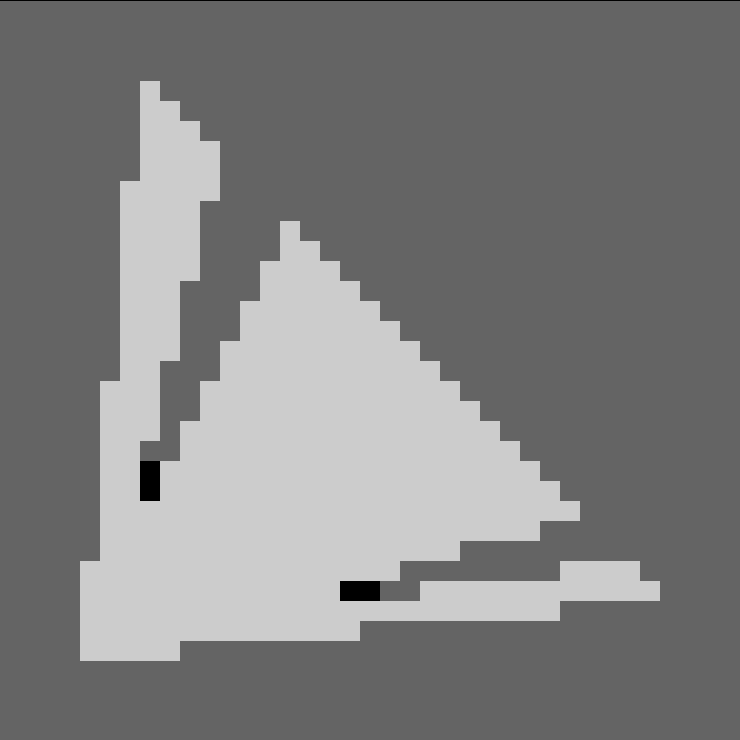
\includegraphics[width=0.3\textwidth]{pictures/testmap.png}\label{fig:maptest}}\hspace{5mm}
\subfloat[Observation model $P(a^i | z_t)$, updating the cells before the detection with $P_\mathrm{free}$ probability, the ones that contain a car with $P_\mathrm{occupied}$ and leaving the ones, covered by the detection untouched.]{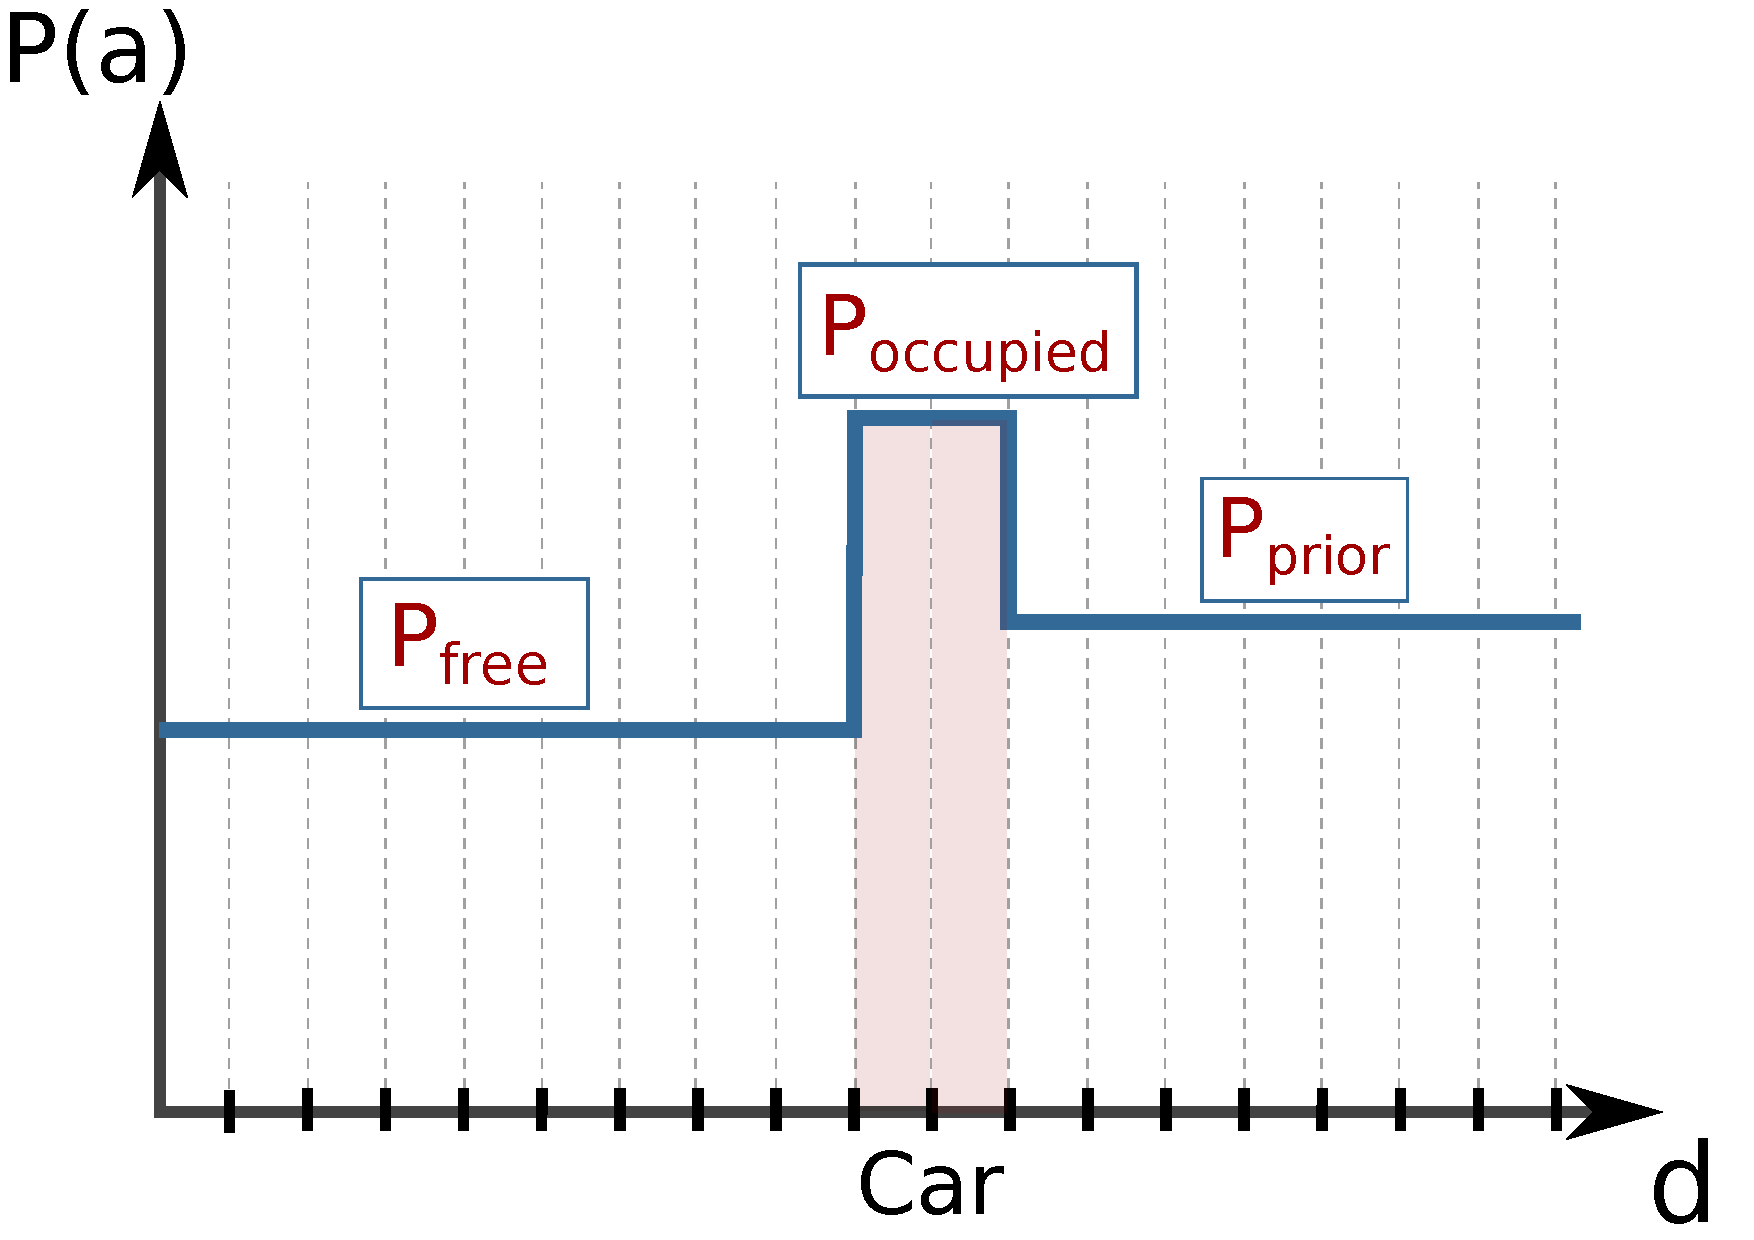
\includegraphics[width=0.65\textwidth]{pictures/observe_model.pdf}\label{fig:observation_model}}
\caption{}
\end{figure}

As presented in Figure~\ref{fig:observation_model}, we define the observation
model along the rays, that span from the camera position to the pre-defined
$d_{\max}$ and along the defined for the camera field of view. In order to
find all the cells of the occupancy grid map that fall into the field of view
of the camera we compute left and right margin points. Following the work
of~\citet{bresenham1965} we search for the cells that form the frontier of the
camera's field of view. The frontier consists of the cells that lie on the
line between the above-mentioned left and right margin points. The margin
points are shown with red circles in Figure~\ref{fig:maptest}.

We carry out the same Bresenham algorithm from the camera cell $c$ to each
query cell $c_i$ in the frontier. Whenever we encounter a cell containing a
car, the next cells within the size of the car are also updated as occupied.
All the ones that come afterwards are not updated as ``not visible''. These
can be seen in an example in Figure~\ref{fig:maptest} as gray ``tails'' behind
the car detections.

We formally define the observation model $P(\v \mid z_t)$ as follows:

\begin{equation}
\label{eq:observation_model}
P(a^i \mid z_t) = \begin{cases} P_{\mathrm{free}}, & \mbox{if } d(c_i) < d(\mathrm{detection}) \\ P_{\mathrm{occupied}}, & \mbox{if } d(\mathrm{detection}) < d(c_i) < d(\mathrm{detection}) + s_{\mathrm{car}} \\ P_{\mathrm{prior}}, & \mbox{if } d(c_i) > d(\mathrm{detection}) + s_{\mathrm{car}} \end{cases}
\end{equation}

where, $d(detection)$ is the distance to the detection point, $d(c_i)$ is the
distance to the $i_\mathrm{th}$ cell, $s_\mathrm{car}$ is the length of the car. We consider
all distances to be measured along the ray from the Bresenham algorithm.

Considering the current setup of the sensor that generates only few
detections, overwhelmed by a number of observations detecting cells as free,
we argue for setting $P_{\mathrm{prior}}$ to 0.5, as we have no prior
knowledge on the occupancy of each cell, $P_{\mathrm{free}}$ to 0.45 to
introduce only a slight update when observing an unoccupied cell and
$P_{\mathrm{occupied}}$ to 0.95 which emulates a high certainty when detecting
an occupied cell.


% subsection occupancy_grids (end)
\subsection{Static State Binary Filter in Pre-defined Positions}
\label{sub:static_state_binary_filter_in_pre_defined_positions}

However, occupancy grids have their drawbacks. One of them, especially for our
setup, is the discretization error. Whenever there are multiple detections of
the same car from different view points it can happen, that the detection is
assigned to different cells of the occupancy grids. This leads to the problem
of data association and therefore difficulties in creating a meaningful
accumulated map.

To avoid the discretization issues we make use of the pre-defined parking lot
positions. These can be set from manual measurements on the ground or from
aerial images. The rest of the theory stays untouched. For each parking lot we
model the occupancy probability likewise to the occupancy grid maps approach
via the static state binary Bayes filter as defined in~\eqref{eq:rec_update}.

The observation model, however, differs significantly from the one used in the
occupancy grip maps. Whenever we detect a parked car, we search for the
closest parking lot and assign the detection to it. The parking lot occupancy
is updated as occupied.

Additionally, we consider the detection of the parked cars to be divided in
sessions. For example, we consider driving near every parking space in the
whole parking area to be one session. The parking lots that were not updated
as occupied during the session are updated as free.

We explicitly stress, that this approach, while needing a pre-processing step
of mapping the parking lots, allows for storing both spacial and occupancy
information in one distinct structure.

% subsection static_state_binary_filter_in_pre_defin (end)
% section model (end)

\section{Action Planning} % (fold)
\label{sec:action_planning}

In this section we formally define the action planning framework that searches
for a path to a free parking lot. It, however, depends on the application what
an optimal solution to this problem is. We therefore explicitly define the
criterium of optimality that we consider throughout this work.

There are typically sub-areas of the parking area, which are better in the
sense of their distance to a common destination. This also means that the
``better'' areas of the parking lots are more likely to be occupied than the
other. An illustration of such situation can be seen in
Figure~\ref{subfig:aerial}. The right part of the parking lot is significantly
more densely occupied than the left one. The relation between the position of
the parking lots and their occupancy leads to a trade-off between driving
straight to the closest-to-goal, but likely occupied parking lot, and parking
in a more distant area, most likely free. It usually takes less time to drive
a car than to walk by foot, but it can take longer to find a free parking lot
closer to the goal than walking from a more distant one. Given the constraints
described above, the framework that we present focuses on finding the solution
that minimizes the expected time spent on finding a free parking lot and
walking from the found one to the goal.

We formally describe the parking as a graph. The states are defined as the set
of vertices $V$, each of which represents a point in $\mathbb{R}^2$. The graph
also has a set of edges $E$ --- a function $V \rightarrow V$, that corresponds
to the actions that can be carried out from one state to another.

\begin{figure}[t]
    \begin{center}
        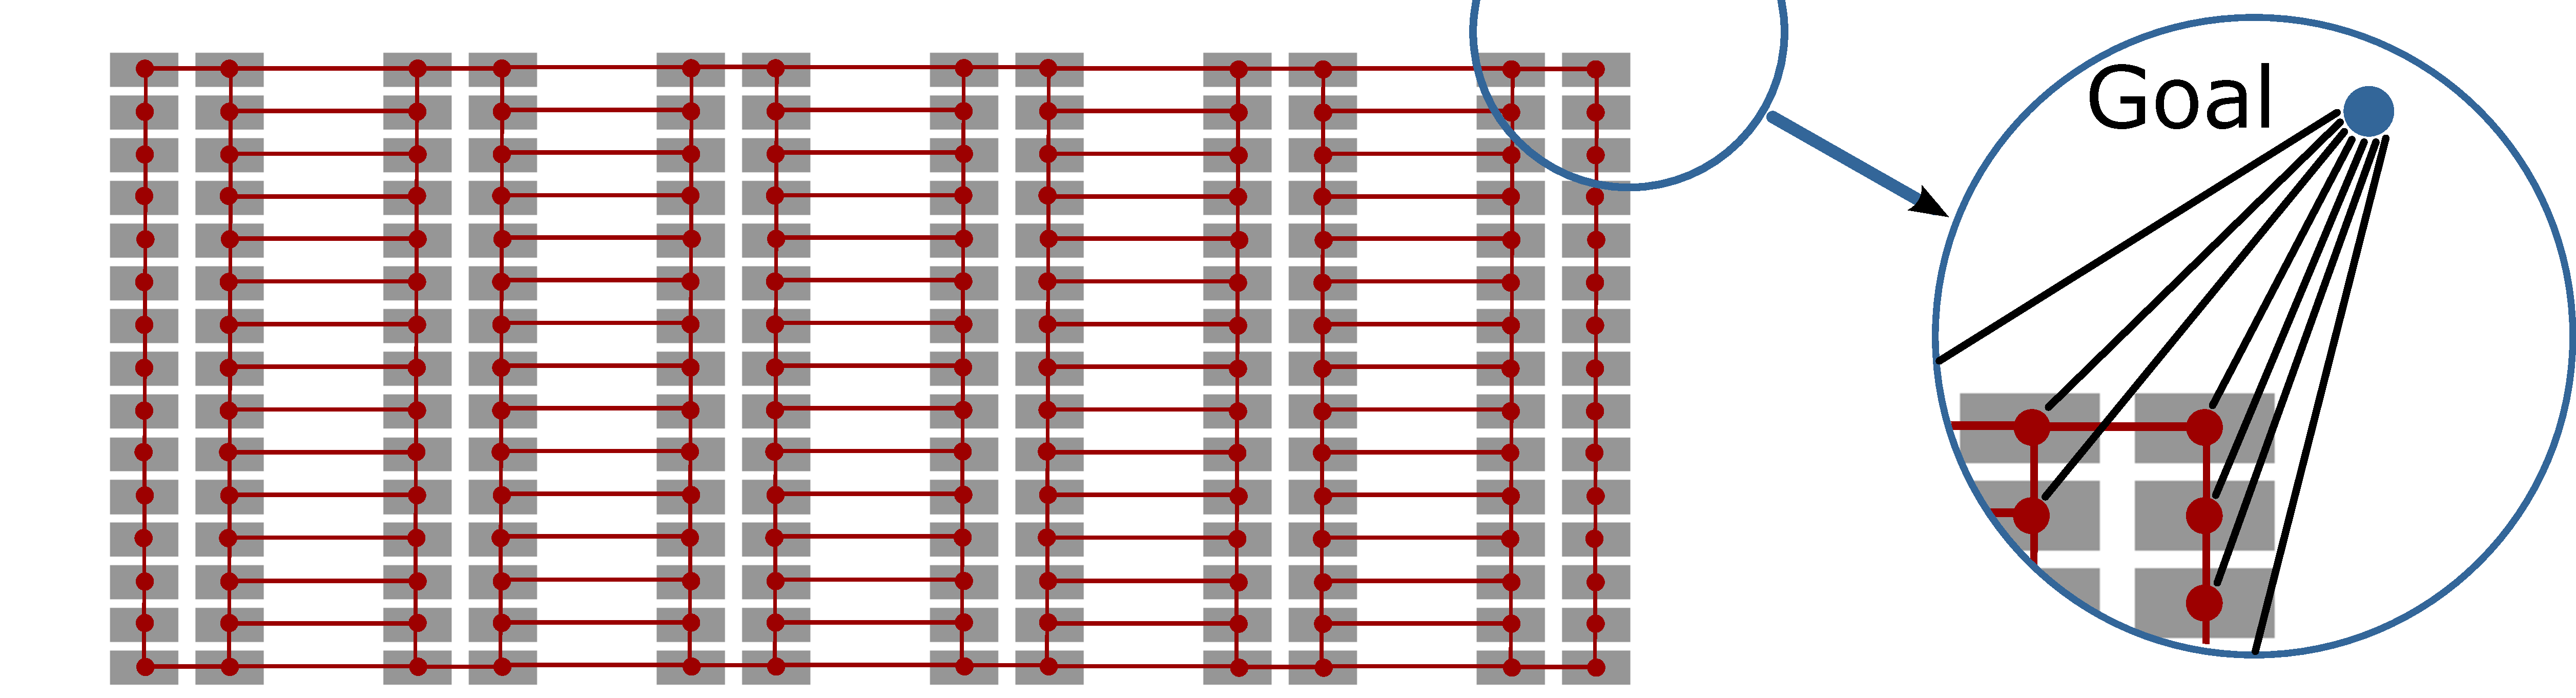
\includegraphics[width=\textwidth]{pictures/graph.pdf}
    \end{center}
    \caption{Graphs based on the parking area. The first graph representation defines different states for positions where the car can drive and the ones where it can only park.
    The second graph is a simplification of the one in the middle. The vertices in it correspond to the parking spaces. The edges between the vertices represent possibilities to reach one state from another, while the actual route is not represented explicitly. The correspondent spacial information is instead stored in the edges. Every state is additionally connected to the goal state.}
    \vspace{-5mm}
    \label{fig:graph}
\end{figure}

In the case where we explicitly map the parking lots --- they, along with
their spacial information, form the vertices of the graph. In this case we
define the edges so that they hold the spacial information about the
connectivity and distances between the parking lots. All vertices are
connected to the goal state. The probability of the action that allows the
agent to follow such edges relies on the occupancy probability of the related
parking lot and is formally defined later.

We also define the set of all actions $A$ that can be carried out in any
state. It consists of five distinct actions: ``up'': $\uparrow$, ``down'':
$\downarrow$, ``left'': $\leftarrow$, ``right'': $\rightarrow$ and ``park''.
Formally:
\begin{eqnarray}
A_{\mathrm{move}} = \{ \uparrow, \downarrow, \leftarrow, \rightarrow \} \\
a_{\mathrm{park}} = \mbox{``park''} \\
A = A_{\mathrm{move}} \cup a_{\mathrm{park}}
\label{eq:actions}
\end{eqnarray}

\citet{tipaldiICRA11} show, that Markov decision processes (MDPs) provide a
way to maximize joint rewards instead of greedily going for the best possible
goal. We follow similar approach, defining rewards and transition
probabilities based on the environment specific to our problem.

Following~\citet{bellman1957}, we define the MDP by the initial state $s_0$,
transition function $T(s \mid s', a)$ and a reward function $R(s, s', a)$.
Here, $T(s \mid s', a)$ denotes the probability of reaching state $s$ if
action $a$ is carried out in state $s'$. The transitions in the model are
assumed to be Markovian. That is, the probability of reaching $s$ from $s'$
depends only on $s'$ and not on the history of earlier states.

For four actions from $A_\mathrm{move}$, we consider the probability of moving
from any state to the next one (if possible) to be equal to 1, while the
probability of parking in a particular state is equal to the occupancy
probability of the state:

\begin{eqnarray}
\forall (s, s') \in E, \forall a \in A_{\mathrm{move}} : \hspace{3mm} T(s \mid s', a) = 1 \\
\forall s \in V, (s,s_{\mathrm{goal}}) \in E : \hspace{3mm} T(s \mid s_{\mathrm{goal}}, a_{\mathrm{park}}) = P(\mathrm{free})
\end{eqnarray}

where $P(\mathrm{free})$ is a probability of a parking lot to be free. To be
consistent, we set the remaining probabilities to the values that guarantee
that $\forall s, s' \in V, (s, s') \in E, \forall a \in A: \sum_{s}T(s \mid
s', a) = 1$. This ensures that in each state the outcome of each action the
agent can take is defined. It resolves to staying in the same state when
trying to carry out an unavailable or improbable action.

For example: it is clear, that staying in the left most corner of the parking
lot and carrying an action to go left, should result in staying in the same
spot and while carrying out an action of parking, with the probability of
$0.6$ there should be a $0.4$ chance to stay in the same place.

We choose the reward function in such way that it guarantees a close relation
between the optimal MDP solution and minimizing the expected time the agent
needs in order to find a free parking lot.

Let route $R$ be an arbitrary path to the destination of interest that the
agent needs to travel to. It is effectively described as a set of edges of the
graph the agent traverses on his way to the goal. Given the transition model
presented above, we argue, that an edge of the graph can be seen as two states
$s_1, s_2$ from $V$ along with an action $a \in A$ such that $T(s_2 \mid s_1,
a) > 0$. We therefore formally define the route as a set of edges with actions
that force the agent to traverse them. The agent starts in the initial state
$s_\mathrm{start}$ and travels to the goal state $s_\mathrm{goal}$. The route
is then:

\begin{equation}
R = \bigcup_{i=\mathrm{start}}^{\mathrm{goal}} \{(s_i, s_{i+1}), a \} \mid (s_i, s_{i+1}) \in E, \exists a: T(s_{i+1} \mid s_i, a) > 0
\end{equation}

This yields the expected time of the route to be defined as:

\begin{equation}
\label{eq:expected_time}
E(t_R) = \sum_{\{(s_i, s_{i+1}), a \} \in R} T(s_{i+1} \mid s_i, a) \cdot t_{s_i, s_{i+1}}
\end{equation}

where $T(s_{i+1} \mid s_i, a)$ is the probability of moving from state $s_i$
to $s_{i+1}$, carrying out action $a$ and $t_{s_i, s_{i+1}}$ is the time it
takes an agent to travel between the defined states.

We seek such route $R^*$ that minimizes the expected time defined in~\eqref{eq:expected_time}:
\begin{equation}
\label{eq:optimal_route}
    R^* = \argmin_R E(t_R)
\end{equation}

Defining the reward function as a decreasing function in time, allows us to
consider a dual problem of finding a route that maximizes the expected reward:

\begin{equation}
    R^* = \argmax_R E(r_R)
\end{equation}

This is a problem that the MDPs are able to solve. We further show the reward
function as a dual representation of agent's travel time and argue on the
differences and similarities between the optimal path provided by MDPs and
$R^*$ as defined in~\eqref{eq:optimal_route}.

The function $R(s, s', a)$, defines the reward for reaching state $s$ from
state $s'$ carrying out action $a$.

We assume, that the agent needs time for driving from one state $s$ to another
$s'$. If he cannot carry out the action and is forced to stay in the same
position, he regardlessly loses time.

The time $t^{s, s'}_\mathrm{drive}$ it takes the agent to drive from any arbitrary state $s$ to an
adjacent one $s'$ depends on the distance between these states and on the
agent's driving speed $v_{\mathrm{drive}}$ and can be defined as:

\begin{equation}
\label{eq:time_to_drive}
\forall s,s' \in V, (s, s') \in E: \hspace{2mm} t_{\mathrm{drive}}^{s,s'}
= \frac{\sqrt{(s - s') {(s - s')}^T}}{v_{\mathrm{drive}}}
\end{equation}

The cost $R(s, s', a)$ of moving from state $s'$ to state $s$ carrying out
action $a$ grows with the time $t_{\mathrm{drive}}^{s,s'}$ the agent needs to
cover the path. We therefore define a negative reward for each action in
$A_{\mathrm{move}}$ between any two adjacent states as follows:

\begin{equation}
\label{eq:drive_reward}
\forall s,s' \in V, \forall (s, s') \in E, \forall a \in A_{\mathrm{move}}: \hspace{2mm} R(s, s', a) = -t_{\mathrm{drive}}^{s,s'}
\end{equation}

In addition to these costs we penalize staying in one place. This cost can
also be seen as the cost of failure. In our system the agent stays in the same
state only if he fails to carry out an optimal action. We define this cost to
be equal to a constant provided beforehand. To show the impact of this cost
let us consider an example. The agent stays in an arbitrary state and thinks
that the best decision in this state is to park. However, when he observes the
parking space --- it is occupied which results in the agent staying in the
same place and as a result, getting the negative reward. Given the fact, that
all rewards in our system are time based this cost virtually results in losing
a pre-defined amount of time.

We also define the rewards that the agent receives when he successfully
carries out parking actions. These rewards are likewise time based. They form
a decreasing linear function in order to guarantee that the state closer to
the destination gets a bigger reward than the one situated further. We define
the reward to be $r_{\max} - r_s$, where $r_s =
t_{\mathrm{walk}}^{s,s_{\mathrm{goal}}}$ is the time that the agent needs to
walk from an arbitrary state $s$ to the goal, $r_{\max} = \max_{s \in V}r_s$
is the greatest of those times. Formally:

\begin{equation}
\label{eq:park_reward}
\forall s \in V, (s, s_{\mathrm{goal}}) \in E : R(s, s_{\mathrm{goal}}, a_{\mathrm{park}}) = r_{\max} - r_s
\end{equation}

To define $r_s$, we define $t_{\mathrm{walk}}^{s,s_{\mathrm{goal}}}$ similarly
to \eqref{eq:time_to_drive}. It depends on the distance between the states $s$ and $s_\mathrm{goal}$ as well as on the walking speed of the agent:

\begin{equation}
t_{\mathrm{walk}}^{s,s_{\mathrm{goal}}} = \frac{\sqrt{(s -
s_{\mathrm{goal}}) {(s - s_{\mathrm{goal}})}^T}}{v_{\mathrm{walk}}}
\end{equation}

The presented reward function $r_{\max} - r_s$ models the win in time between
parking in the worst parking lot and the one represented by state $s$.

The general reward function is fully defined by~\eqref{eq:drive_reward}
and~\eqref{eq:park_reward}. It guarantees, that the agent tries to find a
trade-off between shorter driving and shorter walking paths, weighted by the
occupancy probability of the parking lots.

The key building block of the MDPs is  the utility function, which is a
measure of how good the state is in the long run:

\begin{equation}
\label{eq:non_discount_utility}
U^{\pi}(s) = E\left[\sum_{t=0}^{\infty} R(s_t) \mid \pi,s_0 = s \right]
\end{equation}

Given the definition of the utility function we define the policy as an
expected sum of the rewards obtained, where the expectation is taken over all
possible state sequences that could occur, given that the policy is executed.
The optimal policy $\pi^*$ then satisfies:

\begin{equation}
\label{eq:optimal_policy}
\pi^* = \argmax_\pi \left[ U^{\pi}(s) \mid \pi, s \in \pi \right]
\end{equation}

This equation is, provided the definition of the cost function, effectively
equivalent to~\eqref{eq:optimal_route} leading to $\pi^*$ being an optimal
decision in the means of minimizing the expected time that the agent needs to
find a parking lot.

However, as times goes to infinity the sum in~\eqref{eq:non_discount_utility}
also tends to lean to infinitely big values. In order to avoid this, we make
use of discounted rewards:

\begin{equation}
\label{eq:discount_utility}
U^{\pi}(s) = E\left[\sum_{t=0}^{\infty} \gamma R(s_t) \mid \pi,s_0 = s \right]
\end{equation}

where $\gamma$ is the discount factor --- a number in $[0, 1)$. Formulating
the utility function in such way allows to avoid infinitely big
sums~\cite{Russell:2003:AIM:773294} and allows for searching for the optimal
policy in the way, that we present further in this section. In order to
minimize the deviation of the MDP solution from the one that minimizes the
expected time spent on finding a free parking lot, we set $\gamma$ to a value
close to 1. This, however, results in longer planning times. To deal with this
issue, we utilize the Policy Iteration algorithm that terminates when there is
no update to the policy, omitting estimating exact utility values of all
states.

Policy Iteration algorithm is an iterative algorithm. It alternates the
following two steps, beginning from some initial policy $\pi_0$,

\begin{itemize}
    \item \emph{Policy evaluation:} given a policy $\pi_i$,
    calculate $U_i = U^{\pi_i}$, the utility of each state if $\pi_i$, were to be
    executed.
    \item \emph{Policy improvement:} Calculate a new MEU policy $\pi_{i+1}$, using one-step look-ahead based on
    $U_i$ (as in~\eqref{lbl:optimal_policy}).
\end{itemize}

The \emph{policy evaluation} is performed via solving a linear system of simplified Bellman equations of the form:

\begin{equation}
\label{lbl:bellman_equation}
U(s) = R(s) + \gamma \sum_{s'}T(s \mid s', a)U(s')
\end{equation}

In order to carry out the \emph{policy improvement} step, we choose the
optimal action using the principle of Maximum Expected Utility (MEU) in each
state, that is, choose: the action that maximizes the expected utility of the
subsequent state:

\begin{equation}
\label{lbl:optimal_policy}
\pi^*(s) = \argmax_a \sum_{s'} T(s \mid s', a)U(s')
\end{equation}

The optimal policy $\pi^*(s)$ can be therefore seen as the one that maximizes
the expected utility if followed.

The algorithm terminates when the policy improvement step yields no change in
the utilities. The given method can be shown to converge in $O(n^3)$ where $n$
is the number of vertices in the graph.

This solution to the MDP guarantees to find a route that maximizes the
discounted rewards while searching for the free parking lot and walking from
the found one to the goal. Under the assumption of the discount factor leans
to 1 this route is also the one that minimizes the expected time for searching
for the parking lot.

The agent carries out an optimal strategy to the point when he decides to
park. Let us imagine for a moment that the parking lot at which the agent
wants to park is occupied. From the point of view of the MDPs the optimal
decision would be to wait and try once again, which is clearly a suboptimal
decision. Therefore, we also utilize the observations of the world.

Whenever we move past a parking lot, we check if it is occupied and update
the occupancy probability in the related state to 1 or 0 respectively.
This allows for carrying out a decision based on the better background.

Because the graph is updated, we carry out the policy iteration algorithm
once more to define the new optimal actions for each state.

We repeat this re-planning step until we find a free parking lot.

% section action_planning (end)
